\section{Considera el siguiente P.P.l.}

    \begin{tabular}{|l|l|}
    \hline
        Max & $x_1+2x_2$ \\ \hline
        ~ & $-x_1+3x_2\leq 10$ \\ \hline
        ~ & $x_1+x_2\leq 6$ \\ \hline
        ~ & $x_1-x_2\leq 3$ \\ \hline
        ~ & $x_1+4x_2\geq 4$ \\ \hline
        ~ & $x_1, x_2 \geq 0$ \\ \hline
    \end{tabular}
    \begin{itemize}
        \item Encontrar la solu\'on optima con el met\'odo Simplex(dos fases) 
        
    \begin{tabular}{|l|l|}
    \hline
        Min & $x_7=x_0$ \\ \hline
        ~ & $-x_1+3x_2+x_3 = 10$ \\ \hline
        ~ & $x_1+x_2+x_4 = 6$ \\ \hline
        ~ & $x_1-x_2+x_5 = 3$ \\ \hline
        ~ & $x_1+4x_2-x_6+x_7= 4$ \\ \hline
        ~ & $x_i \geq 0$ \\ \hline
        & $x_3,4,5,6$ variables de holgura \\ \hline
        & $x_7$ variable artiicial \\ \hline
    \end{tabular}        
    
    \textsc{tabla simplex}

\begin{center}
\begin{tabular}{|l|l|l|l|l|l|l|l|l|l|l|}
\hline
   &   & X1 & X2                        & X3 & X4 & X5 & X6 & X7 & RHS &                           \\ \hline
X0 & 1 & -1 & -4                        & 0  & 0  & 0  & 1  & 0  & -4  &                           \\ \hline
X3 & 0 & -1 & 3                         & 1  & 0  & 0  & 0  & 0  & 10  & 3.333333333               \\ \hline
X4 & 0 & 1  & 1                         & 0  & 1  & 0  & 0  & 0  & 6   & 6                         \\ \hline
X5 & 0 & 1  & -1                        & 0  & 0  & 1  & 0  & 0  & 3   & -3                        \\ \hline
X7 & 0 & 1  & \cellcolor[HTML]{67FD9A}4 & 0  & 0  & 0  & -1 & 1  & 4   & \cellcolor[HTML]{67FD9A}1 \\ \hline
\end{tabular}
    
de donde:        

\begin{tabular}{|l|l|l|l|l|l|l|l|l|l|}
\hline
   &   & X1    & X2 & X3 & X4 & X5 & X6    & X7    & RHS                       \\ \hline
X0 & 1 & 0     & 0  & 0  & 0  & 0  & 0     & 1     & \cellcolor[HTML]{32CB00}0 \\ \hline
X3 & 0 & -1.75 & 0  & 1  & 0  & 0  & 0.75  & -0.75 & 7                         \\ \hline
X4 & 0 & 0.75  & 0  & 0  & 1  & 0  & 0.25  & -0.25 & 5                         \\ \hline
X5 & 0 & 1.25  & 0  & 0  & 0  & 1  & -0.25 & 0.25  & 4                         \\ \hline
X2 & 0 & 0.25  & 1  & 0  & 0  & 0  & -0.25 & 0.25  & 1                         \\ \hline
\end{tabular}

existe una soluci\'on

\begin{tabular}{|l|l|l|l|l|l|l|l|l|l|}
\hline
   &   & X1                           & X2 & X3 & X4 & X5 & X6    & RHS &                             \\ \hline
X0 & 1 & -0.5                         & 0  & 0  & 0  & 0  & -0.5  & 2   &                             \\ \hline
X3 & 0 & -1.75                        & 0  & 1  & 0  & 0  & 0.75  & 7   & -4                          \\ \hline
X4 & 0 & 0.75                         & 0  & 0  & 1  & 0  & 0.25  & 5   & 6.666666667                 \\ \hline
X5 & 0 & \cellcolor[HTML]{32CB00}1.25 & 0  & 0  & 0  & 1  & -0.25 & 4   & \cellcolor[HTML]{32CB00}3.2 \\ \hline
X2 & 0 & 0.25                         & 1  & 0  & 0  & 0  & -0.25 & 1   & 4                           \\ \hline
\end{tabular}

\begin{tabular}{|l|l|l|l|l|l|l|l|l|l|}
\hline
   & X0 & X1 & X2 & X3 & X4 & X5   & X6                          & RHS  &                             \\ \hline
   & 1  & 0  & 0  & 0  & 0  & 0.4  & -0.6                        & 3.6  &                             \\ \hline
X3 & 0  & 0  & 0  & 1  & 0  & 1.4  & 0.4                         & 12.6 & 31.5                        \\ \hline
X4 & 0  & 0  & 0  & 0  & 1  & -0.6 & \cellcolor[HTML]{32CB00}0.4 & 2.6  & \cellcolor[HTML]{32CB00}6.5 \\ \hline
X1 & 0  & 1  & 0  & 0  & 0  & 0.8  & -0.2                        & 3.2  & -16                         \\ \hline
X2 & 0  & 0  & 1  & 0  & 0  & -0.2 & -0.2                        & 0.2  & -1                          \\ \hline
\end{tabular}      
        
        \begin{tabular}{|l|l|l|l|l|l|l|l|l|l|}
\hline
   &   & X1 & X2 & X3 & X4  & X5                        & X6 & RHS &                           \\ \hline
X0 & 1 & 0  & 0  & 0  & 1.5 & -0.5                      & 0  & 7.5 & -15                       \\ \hline
X3 & 0 & 0  & 0  & 1  & -1  & \cellcolor[HTML]{32CB00}2 & 1  & 10  & \cellcolor[HTML]{32CB00}5 \\ \hline
X6 & 0 & 0  & 0  & 0  & 2.5 & -1.5                      & 0  & 6.5 & -4.333333333              \\ \hline
X1 & 0 & 1  & 0  & 0  & 0.5 & 0.5                       & 0  & 4.5 & 9                         \\ \hline
X2 & 0 & 0  & 1  & 0  & 0.5 & -0.5                      & 0  & 1.5 & -3                        \\ \hline
\end{tabular}
    
    \begin{tabular}{|l|l|l|l|l|l|l|l|l|}
\hline
   &   & X1 & X2 & X3    & X4   & X5 & X6 & RHS                        \\ \hline
X0 & 1 & 0  & 0  & 0.25  & 1.25 & 0  & 0  & \cellcolor[HTML]{32CB00}10 \\ \hline
X5 & 0 & 0  & 0  & 0.5   & -0.5 & 1  & 1  & 5                          \\ \hline
X6 & 0 & 0  & 0  & 0.75  & 1.75 & 0  & 0  & 14                         \\ \hline
X1 & 0 & 1  & 0  & -0.25 & 0.75 & 0  & 0  & 2                          \\ \hline
X2 & 0 & 0  & 1  & 0.25  & 0.25 & 0  & 0  & 4                          \\ \hline
\end{tabular}    
\end{center}        


    La soluci\'on est\'a dada como\\
    \begin{align}
        x_0=10\\
        x_1=2\\
        x_2=4
    \end{align}
        
        \item Determinar si la soluci\'on optima es \'unica o existen \'optimos alternativos, o bien si el problema no tiene soluciones factibles, o no es acotado
        
        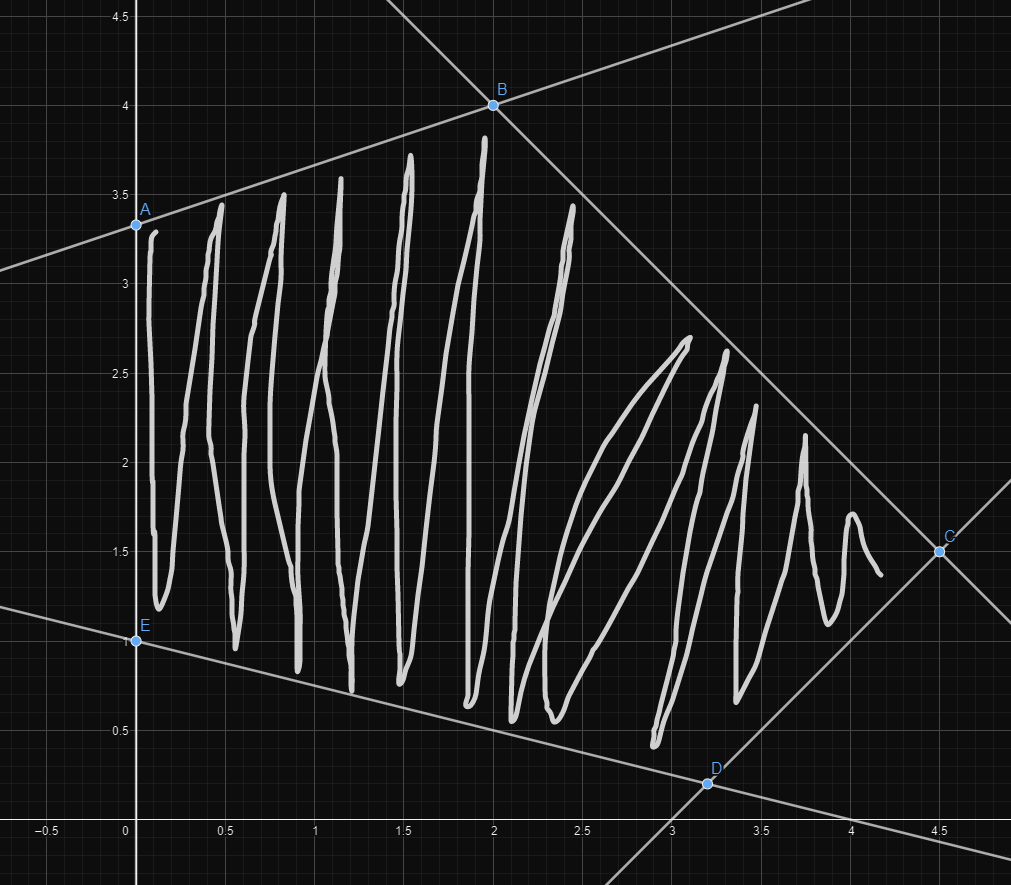
\includegraphics[scale=0.2]{Ejercicios/Imagenes/Ejercicio1b_1.png}\\
        \newpage
        donde:\\

        \begin{align*}
            A=(0,3.33)\\
            B=(2,4)\\
            c=(4.5,1.5)\\
            D=(3.2, 0.2)\\
            E=(0,1)\\
        \end{align*}
        
        Evalundo:
        
                \begin{align*}
            \mbox{Para } A\Rightarrow 0+2(3.33)=6.66\\
            \mbox{Para } B\Rightarrow 2+2(4)=10\\
            \mbox{Para } C \Rightarrow 4.5+2(1.5)=7.5\\
            \mbox{Para } D \Rightarrow 3.2+2(0.2)=3.6\\
            \mbox{Para } E \Rightarrow 0+2(1)=2\\
        \end{align*}
        
        donde el m\'aximo es $10$ para el punto B
        
    \end{itemize}